% Editable, code-aligned replacement for fig:scale. Requires tikz.
\begin{figure}[t]
\centering
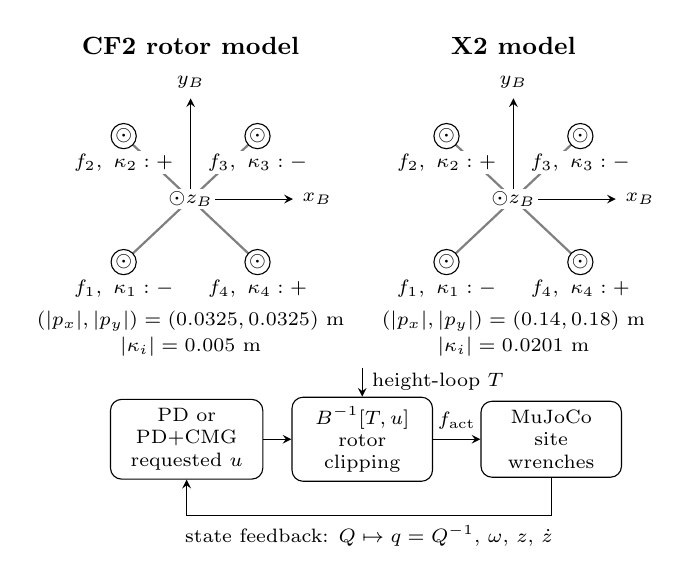
\begin{tikzpicture}[x=1cm,y=1cm,font=\scriptsize,>=stealth]
\foreach \off/\title/\dims/\kap in {0/CF2 rotor model/{0.0325, 0.0325}/0.005,4.1/X2 model/{0.14, 0.18}/0.0201}{
 \begin{scope}[shift={(\off,0)}]
 \node[font=\small\bfseries] at (0,1.95) {\title};
 \draw[gray,thick] (-.85,-.8)--(.85,.8) (-.85,.8)--(.85,-.8);
 \draw[->] (0,0)--(1.3,0) node[right] {$x_B$};
 \draw[->] (0,0)--(0,1.28) node[above] {$y_B$};
 \node[fill=white,inner sep=1pt] at (0,0) {$\odot z_B$};
 \foreach \xx/\yy/\id/\sgn in {-.85/-.8/1/-, -.85/.8/2/+, .85/.8/3/-, .85/-.8/4/+}{
  \draw[fill=white] (\xx,\yy) circle (.16);
  \node at (\xx,\yy) {$\odot$};
  \node[fill=white,inner sep=1pt] at (\xx,\yy-.34) {$f_{\id},\ \kappa_{\id}:\sgn$};
 }
 \node at (0,-1.55) {$(|p_x|,|p_y|)=(\dims)$ m};
 \node at (0,-1.88) {$|\kappa_i|=\kap$ m};
 \end{scope}
}
\node[draw,rounded corners,align=center,text width=1.7cm,minimum height=.75cm] (ctrl) at (-.05,-3.05) {PD or PD+CMG\\requested $\bm u$};
\node[draw,rounded corners,align=center,text width=1.55cm,minimum height=.75cm] (mix) at (2.18,-3.05) {$B^{-1}[T,\bm u\T]\T$\\rotor clipping};
\node[draw,rounded corners,align=center,text width=1.55cm,minimum height=.75cm] (plant) at (4.58,-3.05) {MuJoCo\\site wrenches};
\draw[->] (ctrl)--(mix);
\draw[->] (mix)--node[above] {$\bm f_{\rm act}$}(plant);
\draw[->] (2.18,-2.14)--node[right] {height-loop $T$}(mix.north);
\draw[->] (plant.south)--(4.58,-4.02)--node[below,align=center] {state feedback: $Q\mapsto q=Q^{-1}$, $\bm\omega$, $z$, $\dot z$}(-.05,-4.02)--(ctrl.south);
\end{tikzpicture}
\caption{Code-aligned actuation and feedback interface. Top: body-axis
projections, drawn at independent scales, with rotor numbering matching
the mixer columns. Circles with dots indicate $+z_B$ thrust; $+/-$ labels
give reaction-torque signs, not simulated rotor speeds. X2 site heights
are $0.05$ m for rotors 1--2 and $0.08$ m for 3--4; CF2 sites have zero
height. Bottom: both controllers use the same thrust allocation, clipping,
and state-feedback interface. Table~\ref{tab:models} specifies model authority,
not a manufacturer rating; Table~\ref{tab:manufacturer} provides the hardware comparison.
\eqref{eq:mixer} distinguishes requested from realized wrench.}
\label{fig:scale}
\end{figure}
